\section{Diskussion}
Nedan följer analys av hur projektet har gått och arbetet ur ett vidare perspektiv.  

\subsection{Resultat}

\subsection{Metod}

\subsection{Arbetet i ett vidare sammanhang}
Utöver att projektet har bidragit till vår egen och Saabs nytta kan projektet ha påverkat och ha framtida påverkan på samhället och miljön vi lever i.  

\subsubsection{Etiska och samhälleliga aspekter}
Att utveckla teknik åt ett företag som förser regeringar, myndigheter och företag med militära tjänster och produkter reser många etiska frågor. Hur kan man förhindra att känslig information hamnar i fel händer? Hur kan man veta att användaren har goda avsikter och inte använder vapnen för att förtrycka och förgöra? På Saabs hemsida kan man läsa att de har polisyn noll tolerans mot korruption och att det finns många åtgärder för att uppfylla detta. I figur ~\ref{zerotolerance} visas en grafisk överblick över deras huvudsakliga åtgärder. 
\\
\leavevmode
\begin{figure}[h]
	\centering
	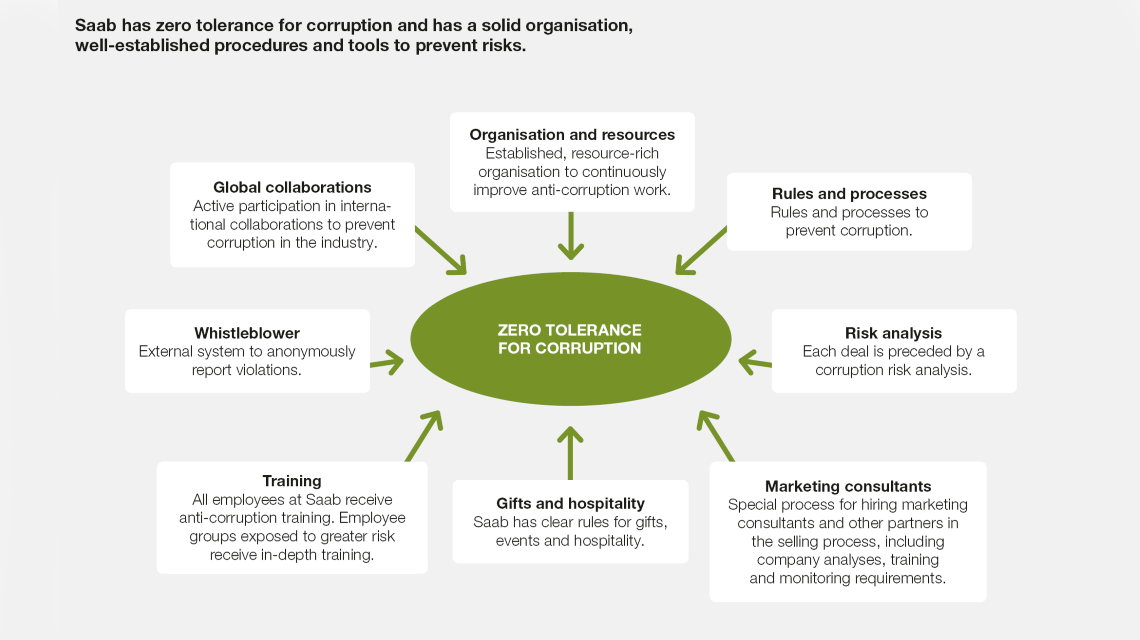
\includegraphics[scale=1.4]{grafik/modell_zero_corruption_1140x640.png}
	\caption{Zero tolerance}\label{fig:zerotolerance}	
\end{figure}  
\\
Till exempel gör Saab alltid riskanalyser i samband med affärer för avgöra om det finns risk för korruption. De undersöker risker med vart affären äger rum, vem köparen är, hur upphandlingen går till och hur köparen kom i kontakt med företaget. Om riskerna inte gick att eliminera eller inte var hanterbara drar sig Saab ur affären. Detta är en åtgärd för att förhindra att produkterna hamnar i fel händer. Ett annat exempel är att Saab ser till att deras etiska värden och riktlinjer strikt följs av utomstående/tillfälligt anställda konsulter och partners. Dessa partners måste genomgå utbildning och lova att följa Saabs etiska värden och riktlinjer. I avtalen ingår det att Saab har rätt till att kontrollera om riktlinjerna verkligen följs. När utomstående parter är iblandade och flödet av pengar inte är helt under Saabs kontroll finns det dock alltid risker men med utbildning och kontroller kan dessa risker minimeras. För att förhindra korruption inom företaget utbildar Saab all personal inom ämnet. De har även ett system kallat "Whistleblower" för att rapportera suspekta aktiviteter som garanterar användarens anonymitet.                 
\\

Det finns alltid en risk med att sälja vapen. I en perfekt värld existerar det inga vapen, vi lever dock inte i en perfekt värld.


\subsubsection{Miljöaspekter}
Flygplan inte speciellt miljövänliga!